\chapter{Buttons and Serial Communications}
\chaplabel{buttons}

\section{Introduction}
This chapter introduces students to using buttons and serial communications.

\section{Buttons}

A typical button circuit is shown in Figure \ref{fig:buttonPullup}. The input is high until the button is pressed.
Unfortunately, being mechanical, buttons do not always create nice, clean switched inputs. Maxim Integrated has a 
\href{https://www.maximintegrated.com/en/design/technical-documents/app-notes/2/287.html}{nice paper} on the topic
advertizing their devices to solve the problem. However, if we don't have the option of adding their hardware, some 
work can be done in software to debounce an input. As Maxim mentions, software debouncing is not free. It does incur
some overhead so you probably do not want to do it for many inputs. Am example of software debouncing is in 
Listing \ref{lst:debounce}.

\begin{lstlisting}[language=C++, caption={This is the Arduino example of software debouncing.},label={lst:debounce}]
	/*
	Debounce
  
	Each time the input pin goes from LOW to HIGH (e.g. because of a push-button
	press), the output pin is toggled from LOW to HIGH or HIGH to LOW. There's a
	minimum delay between toggles to debounce the circuit (i.e. to ignore noise).
  
	The circuit:
	- LED attached from pin 13 to ground through 220 ohm resistor
	- pushbutton attached from pin 2 to +5V
	- 10 kilohm resistor attached from pin 2 to ground
  
	- Note: On most Arduino boards, there is already an LED on the board connected
	  to pin 13, so you don't need any extra components for this example.
  
	created 21 Nov 2006
	by David A. Mellis
	modified 30 Aug 2011
	by Limor Fried
	modified 28 Dec 2012
	by Mike Walters
	modified 30 Aug 2016
	by Arturo Guadalupi
  
	This example code is in the public domain.
  
	https://www.arduino.cc/en/Tutorial/BuiltInExamples/Debounce
  */
  
  // constants won't change. They're used here to set pin numbers:
  const int buttonPin = 9;    // the number of the pushbutton pin
  const int ledPin = 13;      // the number of the LED pin
  
  // Variables will change:
  int ledState = LOW;         // the current state of the output pin
  int buttonState;             // the current reading from the input pin
  int lastButtonState = LOW;   // the previous reading from the input pin
  
  // the following variables are unsigned longs because the time, measured in
  // milliseconds, will quickly become a bigger number than can be stored in an int.
  unsigned long lastDebounceTime = 0;  // the last time the output pin was toggled
  unsigned long debounceDelay = 50;    // the debounce time; increase if the output flickers
  
  void setup() {
	Serial.begin(115200);
	while(!Serial) delay(10);
	Serial.println("Starting...");
	
	pinMode(buttonPin, INPUT);
	pinMode(ledPin, OUTPUT);
  
	// set initial LED state
	digitalWrite(ledPin, ledState);
  }
  
  void loop() {
	// read the state of the switch into a local variable:
	int reading = digitalRead(buttonPin);
  
	// check to see if you just pressed the button
	// (i.e. the input went from LOW to HIGH), and you've waited long enough
	// since the last press to ignore any noise:
  
	// If the switch changed, due to noise or pressing:
	if (reading != lastButtonState) {
	  // reset the debouncing timer
	  lastDebounceTime = millis();
	}
  
	if ((millis() - lastDebounceTime) > debounceDelay) {
	  // whatever the reading is at, it's been there for longer than the debounce
	  // delay, so take it as the actual current state:
  
	  // if the button state has changed:
	  if (reading != buttonState) {
		buttonState = reading;
  
		// only toggle the LED if the new button state is HIGH
		if (buttonState == HIGH) {
		  ledState = !ledState;
		}
	  }
	}
  
	// set the LED:
	digitalWrite(ledPin, ledState);
  
	// save the reading. Next time through the loop, it'll be the lastButtonState:
	lastButtonState = reading;
  
  }
\end{lstlisting}

\begin{figure}[!htb]
	\centering
	\includegraphics{buttonSerial/button1.eps}
	\label{fig:buttonPullup}
	\caption{This is a typical button input circuit.}
\end{figure}

\begin{figure}[!htb]
	\centering
	\includegraphics[scale=0.5]{buttonSerial/debounce.eps}
	\label{fig:buttonDebounce}
	\caption{This is an example of what the output signal from a button with the circuit in Figure \ref{fig:buttonPullup} could look like.}
\end{figure}


\section{Types of Serial}

\begin{figure}[!htb]
	% Serial
	\centering
	\begin{tikzpicture}
		% BLOCKS
		\draw[thick] (0,0) rectangle (4,4) node (dev1) [pos=0.5] {Device 1};
		\draw[thick] (8,0) rectangle (12,4) node (dev2) [pos=0.5] {Device 2};
		% ARROWS	
		\draw [thick,-{latex[length=4mm, width=6mm]}] (4,2) |- node [above,pos=0.75] {01101101} (8,2) ;
	\end{tikzpicture}
	\label{fig:serial}
	\caption{Serial transfers one bit at a time.}
\end{figure}
	
	% Parallel
\begin{figure}[!htb]
	\centering
	\begin{tikzpicture}
		% BLOCKS
		\draw[thick] (0,0) rectangle (4,5) node (dev3) [pos=0.5] {Device 1};
		\draw[thick] (8,0) rectangle (12,5) node (dev4) [pos=0.5] {Device 2};
		% ARROWS	
		\draw [thick,-{latex[length=4mm, width=6mm]}] (4,4.25) |- node [above,pos=0.75] {0} (8,4.25) ;
		\draw [thick, -{latex[length=4mm, width=6mm]}] (4,3.75) |- node [above,pos=0.75] {1} (8,3.75) ;
		\draw [thick, -{latex[length=4mm, width=6mm]}] (4,3.25) |- node [above,pos=0.75] {1} (8,3.25) ;
		\draw [thick, -{latex[length=4mm, width=6mm]}] (4,2.75) |- node [above,pos=0.75] {0} (8,2.75) ;
		\draw [thick, -{latex[length=4mm, width=6mm]}] (4,2.25) |- node [above,pos=0.75] {1} (8,2.25) ;
		\draw [thick, -{latex[length=4mm, width=6mm]}] (4,1.75) |- node [above,pos=0.75] {1} (8,1.75) ;
		\draw [thick, -{latex[length=4mm, width=6mm]}] (4,1.25) |- node [above,pos=0.75] {0} (8,1.25) ;
		\draw [thick, -{latex[length=4mm, width=6mm]}] (4,0.75) |- node [above,pos=0.75] {1} (8,0.75) ;
		
	\end{tikzpicture}
	\label{fig:parallel}
	\caption{Parallel transfers multiple bits at a time.}
\end{figure}

\begin{figure}[!htb]
	% UART
	\centering
	\begin{tikzpicture}
		% BLOCKS
		\draw[thick] (0,0) rectangle (4,4) node (dev1) [pos=0.5] {Device 1};
		\draw[thick] (8,0) rectangle (12,4) node (dev2) [pos=0.5] {Device 2};
		% ARROWS	
		\draw [thick,-{latex[length=4mm, width=6mm]}] (4,2.5) node [anchor=east] {TX} -- (8,1.5) node [anchor=west] {RX} ;
		\draw [thick,{latex[length=4mm, width=6mm]}-] (4,1.5) node [anchor=east] {RX} -- (8,2.5) node [anchor=west] {TX} ;
	\end{tikzpicture}
	\label{fig:uart}
	\caption{A UART has full duplex between two entities.}
\end{figure}

\begin{figure}[!htb]
	% SPI
	\centering
	\begin{tikzpicture}
		% BLOCKS
		\draw[thick] (0,0) rectangle (4,4) node (dev1) [pos=0.5] {Controller};
		\draw[thick] (8,0) rectangle (12,4) node (dev2) [pos=0.5] {Peripheral 1};
		\draw[thick] (8, -2) rectangle (12,-6) node (dev3) [pos=0.5] {Peripheral 2};
		% ARROWS	
		\draw [thick,-{latex[length=4mm, width=6mm]}] (4,2.5) node [anchor=east] {COPI} -- (8,2.5) node [anchor=west] {COPI} ;
		\draw [thick,{latex[length=4mm, width=6mm]}-] (4,1.5) node [anchor=east] {CIPO} -- (8,1.5) node [anchor=west] {CIPO} ;
		\fill[black]  (6,1.5) circle (3pt) ;
		\draw [thick] (6,1.5) |- (8,-3.5) node [anchor=west] {CIPO} ;
		\draw [thick, -{latex[length=4mm, width=6mm]}] (7,2.5) |- (8,-2.5) node [anchor=west] {COPI} ;
		\fill[black]  (7,2.5) circle (3pt) ;
		\draw [thick,-{latex[length=4mm, width=6mm]}] (4,3.5) node [anchor=east] {CS1} |- (8,3.5) node [anchor=west] {CS} ;
		\draw [thick,-{latex[length=4mm, width=6mm]}] (4,0.5) node [anchor=east] {CS2} |- (5,0.5) |- (8,-4.5) node [anchor=west] {CS} ;
	\end{tikzpicture}
	\label{fig:spi}
	\caption{SPI allows for one (sometime more) controller and multiple peripherals.}
\end{figure}

\begin{figure}[!htb]
	% I2C
	\centering
	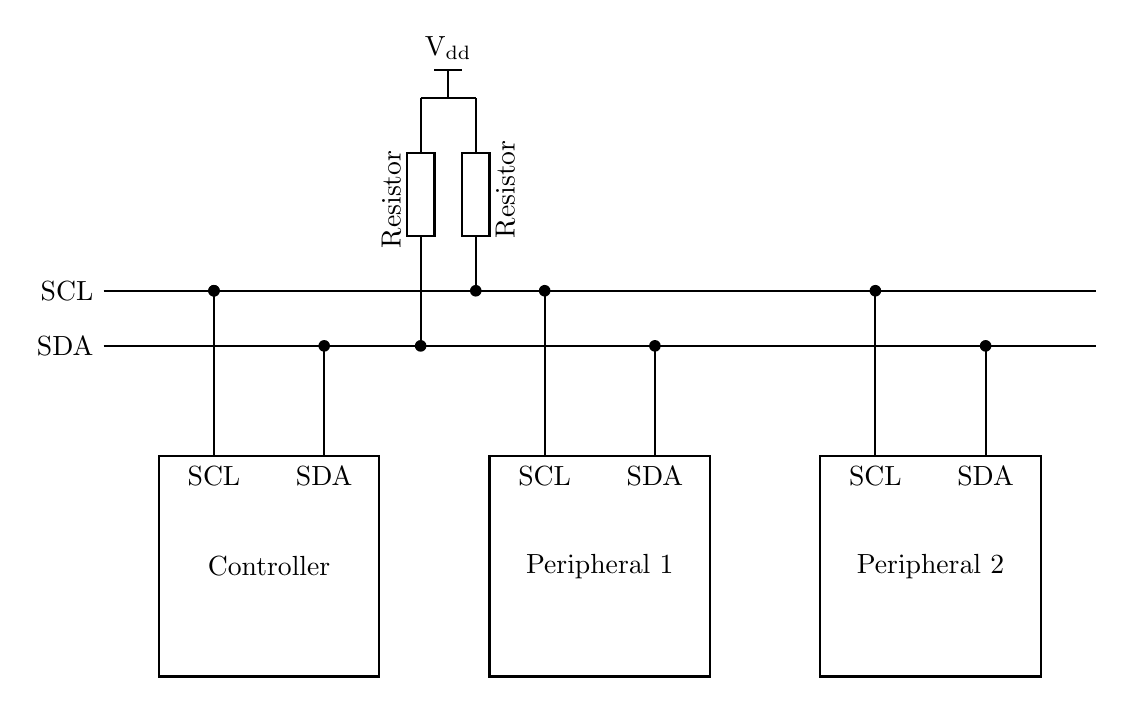
\begin{tikzpicture}[scale=0.7]
		% BLOCKS
		\draw[thick] (0,0) rectangle (4,4) node (dev1) [pos=0.5] {Controller};
		\draw[thick] (6,0) rectangle (10,4) node (dev2) [pos=0.5] {Peripheral 1};
		\draw[thick] (12, 0) rectangle (16,4) node (dev3) [pos=0.5] {Peripheral 2};
		\draw[thick] (4.5, 8) rectangle (5,9.5) node (r1) [above=2ex,pos=0.15, rotate=90] {Resistor};
		\draw[thick] (5.5, 8) rectangle (6,9.5) node (r2) [below=2ex,pos=0.85, rotate=90] {Resistor};
		
		% ARROWS	
		\draw [thick] (-1,6) node [anchor=east] {SDA} -- (17,6) ;
		\draw [thick] (-1,7) node [anchor=east] {SCL} -- (17,7)  ;
		\draw [thick] (1,4) node [anchor=north] {SCL} -- (1,7) ;
		\draw [thick] (3,4) node [anchor=north] {SDA} -- (3,6) ;
		\draw [thick] (7,4) node [anchor=north] {SCL} -- (7,7) ;
		\draw [thick] (9,4) node [anchor=north] {SDA} -- (9,6) ;
		\draw [thick] (13,4) node [anchor=north] {SCL} -- (13,7) ;
		\draw [thick] (15,4) node [anchor=north] {SDA} -- (15,6) ;
		\fill[black]  (1,7) circle (3pt) ;
		\fill[black]  (1,7) circle (3pt) ;
		\fill[black]  (7,7) circle (3pt) ;
		\fill[black]  (13,7) circle (3pt) ;
		\fill[black]  (3,6) circle (3pt) ;
		\fill[black]  (9,6) circle (3pt) ;
		\fill[black]  (15,6) circle (3pt) ;
		\draw [thick] (4.75,6)  -- (4.75,8) ;
		\fill[black]  (4.75,6) circle (3pt) ;
		\draw [thick] (5.75,7)  -- (5.75,8) ;
		\fill[black]  (5.75,7) circle (3pt) ;
		\draw [thick] (5.75,9.5)  -- (5.75,10.5) ;
		\draw [thick] (4.75,9.5)  -- (4.75,10.5) ;
		\draw [thick] (4.75,10.5)  -- (5.75,10.5) ;
		\draw [thick] (5.25,10.5)  -- (5.25,11) ;
		\draw [thick] (5,11)  -- node [above,pos=0.5] {V\textsubscript{dd}} (5.5,11) ;
	\end{tikzpicture}
	\label{fig:i2c}
	\caption{I\textsuperscript{2}C allows for multiple controllers and peripherals on the same bus.}
\end{figure}


\section{I2C}
I2C addresses for modules that are on the board or may be used with the board can be seen in Table \ref{table:i2caddresses}.

\begin{table}[!ht]
	\centering
	\begin{tabular}{l l}
		\hline
		Address (HEX) & Module \\ 
		\hline
		0x44 or 0x45 & SHT31-DIS Temperature/Humidity \\
		0x3D & 1.3" 128x64 OLED Display \\
		0x39 & APDS-9960 Light, Color, Proximity, Gesture \\
		0x77 & BME688 Temperature, Humidity, Gas \\
		0x2D, 0x53, and 0x57 & ST25DV16 Dynamic NFC/RFID Tag IC \\
		0x30 or other  & NeoKey 1x4 QT breakout board \\
		0x10 & STEMMA MiniGPS \\
		\hline
	\end{tabular}
	\caption{I2C addresses for relevant modules.}
	\label{table:i2caddresses}
\end{table}